\chapter{Evaluation Synthesis and Discussion}\label{cpt:discussion}

The dissertation is best read as one research line rather than five independent demonstrations. CodeMarkBench defines an executable denominator; SemCodebook turns the benchmark lesson into structured white-box provenance; CodeDye shows what remains auditable when model internals disappear; ProbeTrace adds an owner registry for source-bound attribution; and SealAudit asks whether watermark evidence should trigger security review. This chapter compares those stages without forcing them into one weighted score.

\section{Synthesis Protocol}

The synthesis uses three rules. First, a result is interpreted through the evidence object it actually measures. A 97.26\% SemCodebook recovery rate and a 2.00\% CodeDye sparse-signal rate are not competing accuracies: one is a white-box provenance recovery event, and the other is a black-box null-audit event. Second, strong-looking numbers are paired with controls or abstentions. ProbeTrace's 300/300 APIS result is read with false-owner controls and single-owner scope; SealAudit's 0 unsafe-pass observation is read with high needs-review coverage. Third, support-only evidence remains non-promoting. Ablations, transfer rows, visible-marker diagnostics, and continuation plans may motivate later work, but they do not alter a submitted denominator.

These rules fit source-code watermarking because a generated program is not merely a string, and a detector output is not automatically provenance, ownership, contamination evidence, or safety evidence. Each transition in WatermarkScope changes either access or risk: executable benchmark rows become inspectable carriers, carriers become preserved transcripts, transcripts become owner-bound witnesses, and owner-bound evidence becomes marker-hidden triage. The useful question is therefore whether each stage reports the strongest claim supported by its access model.

\section{Cross-Stage Result Surface}

Table~\ref{tab:main-results} is the compressed result surface of the dissertation. It is not a leaderboard. The columns identify the counted object, the observed outcome, and the strongest reading that survives the controls.

\begin{table}[htbp]
\centering
\caption{Main quantitative result surfaces. Denominators are fixed within modules and are not interchangeable across modules.}
\label{tab:main-results}
\tighttable
\begin{tabularx}{\textwidth}{@{}L{1.72cm}L{2.35cm}L{2.95cm}Y@{}}
\toprule
Lifecycle stage & Main denominator & Observation & Safe reading \\
\midrule
Benchmark & 140 model-method-source runs & 140/140 complete; no method dominates all dimensions. & Finite executable release matrix. \\
Provenance & 24,000 positives; 48,000 negatives & 23,342 recovered; 0 negative hits. & Admitted-cell white-box provenance evidence. \\
Audit & 300 live rows plus fixed controls & 6 sparse live signals; 170/300 positive controls; 0/300 negative controls. & Null audit, not prevalence. \\
Attribution & 300 APIS rows; 1,200 false-owner controls & 300 scoped attributions; 0 false-owner hits. & Single active owner only. \\
Triage & 960 marker-hidden rows & 81 decisive; 879 needs review; 0 unsafe pass. & Selective triage, not a certificate. \\
\bottomrule
\end{tabularx}
\end{table}

A single scalar would be misleading. It would either reward CodeDye for sparse signals that are not prevalence evidence, or penalize SealAudit for abstaining even though abstention is the conservative action. The dissertation instead reports a vector: denominator, observation, controls, uncertainty, and excluded interpretation. Appendix~\ref{app:artifact-index}, Table~\ref{tab:support-only-ledger}, records the exclusion ledger used to check those boundaries.

\begin{figure}[htbp]
  \centering
  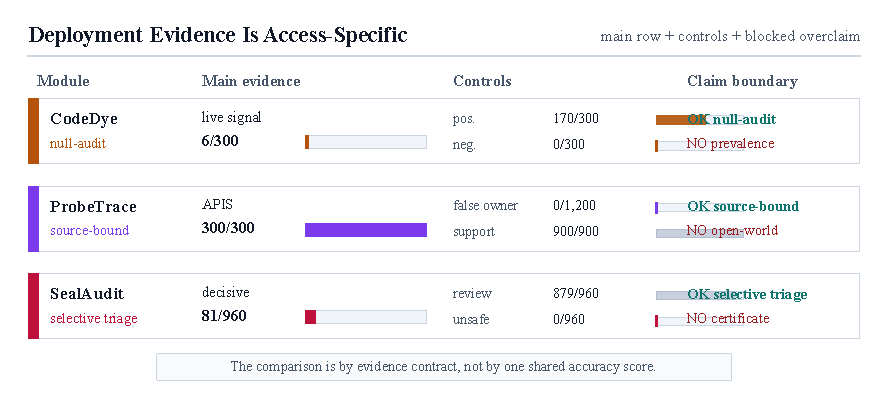
\includegraphics[width=\textwidth]{fig/blackbox_outcomes.pdf}
  \caption{Deployment-facing evidence contracts for sparse audit, scoped attribution, and selective triage. These are access-specific result surfaces, not comparable detector accuracies.}
  \label{fig:blackbox-outcomes}
\end{figure}

Figure~\ref{fig:blackbox-outcomes} makes the deployment contrast visible. CodeDye has low live yield, but positive and negative controls show that the audit predicate is not arbitrary. ProbeTrace is numerically strong because the owner registry and source split are fixed. SealAudit is intentionally abstention-heavy: most cases are routed to review, while unsafe pass-through remains the protected failure mode.

\begin{figure}[htbp]
  \centering
  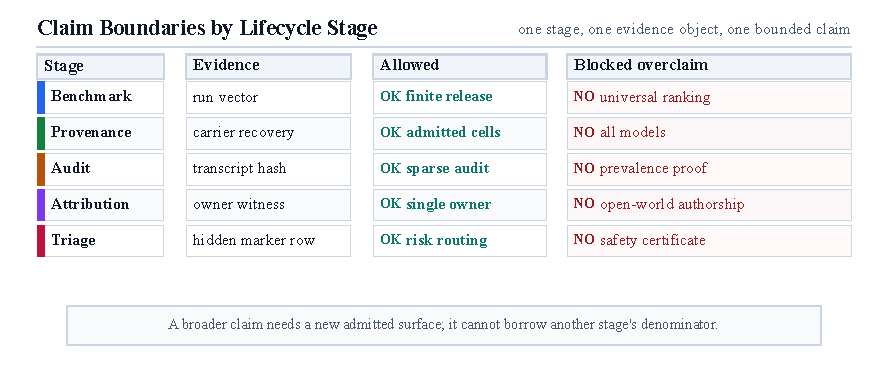
\includegraphics[width=\textwidth]{fig/claim_boundary_matrix.pdf}
  \caption{Claim boundaries across the lifecycle. The blocked-overclaim column is part of the method, not a footnote.}
  \label{fig:claim-boundary-matrix}
\end{figure}
\FloatBarrier

Figure~\ref{fig:claim-boundary-matrix} states the same rule visually. Every stage has an evidence object, an allowed reading, and a blocked overclaim. If later work adds a model family, provider, owner setting, or triage rule, it should create a new denominator rather than silently expanding the old one.

The two figures should therefore be read as complements rather than as repeated summaries. Figure~\ref{fig:blackbox-outcomes} shows why the three deployment-facing modules are not comparable by raw success rate: their rows represent different events. Figure~\ref{fig:claim-boundary-matrix} then records the stronger governance rule: a claim is admissible only inside the stage whose evidence object produced it. This is the synthesis contribution of WatermarkScope. The framework is not a weighted average of five systems; it is a set of constraints for deciding which result is allowed to mean what.

\section{Lessons Across Access Models}

The benchmark lesson is that executable evaluation changes the meaning of a watermark score. CodeMarkBench reports 140/140 canonical run completion, but that number is an inventory-completion result, not detector success. The scientific content is in component behavior: robustness, utility, release completeness, negative controls, and efficiency. This discipline carries into the later modules: SemCodebook keeps its 658 miss, abstain, or reject outcomes inside the positive denominator; CodeDye keeps no-signal rows inside the live audit denominator; ProbeTrace does not treat 900 transfer rows as primary APIS attributions; and SealAudit reports needs-review outcomes rather than hiding them behind accuracy.

The access-model lesson is that confidence cannot be transferred across stages. Under white-box access, SemCodebook can inspect typed carriers, validate helper closure, and recover an identifier with ECC-style decoding, schedule commitments, and positive-support evidence. Under black-box provider access, CodeDye cannot recover the same evidence object, so it preserves transcript-bound audit evidence instead. Under an owner-registry setting, ProbeTrace can make a stronger source-bound claim, but only because the active owner and source split are fixed before evaluation. Under security triage, SealAudit gives up broad classification coverage in exchange for an explicit unsafe-pass boundary.

The governance lesson is that watermarking systems need reviewable evidence, not only automatic labels. CodeDye is useful even with a sparse signal because it preserves rows for review without making an accusation. ProbeTrace distinguishes source-bound attribution from generic similarity. SealAudit turns ambiguous cases into explicit review work instead of forcing labels. These choices do not maximize one metric, but they avoid unsupported conclusions.

\section{Validity and Reproducibility}

Every rate in the dissertation is reported with a numerator, denominator, and claim boundary. For zero-event controls, the correct interpretation is not zero risk; it is 0 observed events with a nonzero upper confidence bound. For example, SemCodebook's 0/48,000 negative-control hits support a tight false-positive bound within the evaluated surface, while ProbeTrace's 0/1,200 false-owner controls support only the scoped owner protocol. For clustered evidence, such as ProbeTrace transfer rows, the primary independence unit remains the task cluster rather than the raw row count.

The principal internal-validity risk is outcome-dependent selection. The dissertation addresses it by separating claim-bearing rows from support-only rows and by recording denominator boundaries in manifests. The principal external-validity risk is that future models, providers, languages, attacks, or owner settings may behave differently. The response is denominator continuity: new model cells, providers, owner registries, or triage reruns should create new result surfaces rather than silently broadening the submitted FYP claims. The principal construct-validity risk is using the wrong metric for the question. Accuracy is not the right metric for SealAudit because abstention is designed; a weighted score is not the right metric for the lifecycle because recovery, audit yield, attribution, and triage coverage are different constructs.

The submitted code package supports this interpretation. The examiner-facing scripts verify that written claims are traceable to preserved result manifests, canonical artifacts, and claim-boundary files. They do not require a full GPU/API rerun inside the dissertation build. The report therefore separates three reproducibility layers: executable reruns for benchmark and local code, artifact reconstruction for preserved experiment outputs, and audit traceability for black-box transcripts or adjudicated rows.

The same separation explains the future-work plan. A new SemCodebook model family should not modify the reported 24,000-positive denominator; it should create a new admitted-cell surface. A new CodeDye provider should not be merged into the 300 DeepSeek rows; it should receive a provider-specific frozen audit surface and control suite. A future ProbeTrace multi-owner setting should add simultaneous-owner margins and owner-heldout controls before claiming broader attribution. A future SealAudit resolver should improve coverage only if it preserves the unsafe-pass event definition. These continuation rules are operational safeguards against overfitting because they prevent a later successful slice from rewriting the original denominator.

\section{Conclusion}

The research question asked how source-code watermarking can be evaluated, embedded, traced, and audited under realistic code-generation conditions. WatermarkScope answers it as an evidence chain: executable benchmarks expose reliability gaps, structured carriers support white-box provenance, black-box and owner-bound protocols preserve traceable evidence, and security triage audits marker-hidden risk. The completed FYP contribution is a benchmark-to-audit framework with code, artifacts, reproducible manifests, and conservative statistical reporting. Its central result is the evidence contract: as access weakens and risk changes, the claim must change with the evidence object.

The practical standard left by the dissertation is simple: future experiments should add denominators rather than quietly broadening old claims. A benchmark paper can expand CodeMarkBench with a new versioned matrix; a SemCodebook paper can admit new model cells; CodeDye can add provider-specific frozen controls; ProbeTrace can broaden registered owner surfaces; and SealAudit can improve coverage while preserving unsafe-pass accounting. These continuations are separated in Appendix~\ref{app:publication-plan}, but they share one rule: source-code watermarking becomes scientifically useful only when evidence, access, risk, and abstention are reported together.

For that reason, the final artifact should be judged as an evidence framework rather than as a collection of isolated prototypes. Its contribution is the combination of executable benchmarking, structured provenance, black-box audit preservation, source-bound attribution, and selective security triage under one reproducibility discipline. The strongest future version of the work is not obtained by making every number look larger; it is obtained by admitting new surfaces before measuring them, keeping weak or ambiguous outcomes visible, and letting the claim boundary change whenever access or risk changes.
